%%%%%%%%%%%%%%%%%%%%%%%%%%%%%%%%%%%%%%%%%
%  My documentation report
%  Objetive: Explain what I did and how, so someone can continue with the investigation
%
% Important note:
% Chapter heading images should have a 2:1 width:height ratio,
% e.g. 920px width and 460px height.
%
%%%%%%%%%%%%%%%%%%%%%%%%%%%%%%%%%%%%%%%%%

%----------------------------------------------------------------------------------------
%	PACKAGES AND OTHER DOCUMENT CONFIGURATIONS
%----------------------------------------------------------------------------------------

\documentclass[11pt,fleqn]{book} % Default font size and left-justified equations

\usepackage[top=3cm,bottom=3cm,left=3.2cm,right=3.2cm,headsep=10pt,a4paper]{geometry} % Page margins


\usepackage{xcolor} % Required for specifying colors by name
\definecolor{ocre}{RGB}{52,177,201} % Define the orange color used for highlighting throughout the book

% Font Settings
\usepackage{avant} % Use the Avantgarde font for headings
%\usepackage{times} % Use the Times font for headings
\usepackage{mathptmx} % Use the Adobe Times Roman as the default text font together with math symbols from the Sym­bol, Chancery and Com­puter Modern fonts

\usepackage{microtype} % Slightly tweak font spacing for aesthetics




% Bibliography
\usepackage[style=alphabetic,sorting=nyt,sortcites=true,autopunct=true,babel=hyphen,hyperref=true,abbreviate=false,backref=true,backend=biber]{biblatex}
\addbibresource{bibliography.bib} % BibTeX bibliography file
\defbibheading{bibempty}{}

%----------------------------------------------------------------------------------------
%	VARIOUS REQUIRED PACKAGES
%----------------------------------------------------------------------------------------

\usepackage{titlesec} % Allows customization of titles

\usepackage{graphicx} % Required for including pictures
\graphicspath{{Pictures/}} % Specifies the directory where pictures are stored

\usepackage{lipsum} % Inserts dummy text

\usepackage{tikz} % Required for drawing custom shapes
\usepackage[utf8]{inputenc} % Required for including letters with accents
\usepackage[T1]{fontenc} % Use 8-bit encoding that has 256 glyphs

\usepackage[russian]{babel}

\usepackage{enumitem} % Customize lists
\setlist{nolistsep} % Reduce spacing between bullet points and numbered lists

\usepackage{booktabs} % Required for nicer horizontal rules in tables

\usepackage{eso-pic} % Required for specifying an image background in the title page

%----------------------------------------------------------------------------------------
%	MAIN TABLE OF CONTENTS
%----------------------------------------------------------------------------------------

\usepackage{titletoc} % Required for manipulating the table of contents

\contentsmargin{0cm} % Removes the default margin

% part text styling
\titlecontents{part}[0cm] % Indentation
{\addvspace{18pt}\large\sffamily\bfseries\color{ocre}\contentslabel[\Large\thecontentslabel]{1.25cm}} % Spacing and font options for chapters
{\color{ocre!60}\contentslabel[\Large\thecontentslabel]{1.25cm}\color{ocre}} % Chapter number
{}  
{\color{ocre!60}\normalsize\sffamily\bfseries\;\titlerule*[.5pc]{.}\;\thecontentspage} % Page number




% Chapter text styling
\titlecontents{chapter}[1.25cm] % Indentation
{\addvspace{15pt}\large\sffamily\bfseries} % Spacing and font options for chapters
{\color{ocre!60}\contentslabel[\Large\thecontentslabel]{1.25cm}\color{ocre}} % Chapter number
{}  
{\color{ocre!60}\normalsize\sffamily\bfseries\;\titlerule*[.5pc]{.}\;\thecontentspage} % Page number
% Section text styling
\titlecontents{section}[1.25cm] % Indentation
{\addvspace{5pt}\sffamily\bfseries} % Spacing and font options for sections
{\contentslabel[\thecontentslabel]{1.25cm}} % Section number
{}
{\sffamily\hfill\color{black}\thecontentspage} % Page number
[]
% Subsection text styling
\titlecontents{subsection}[1.25cm] % Indentation
{\addvspace{1pt}\sffamily\small} % Spacing and font options for subsections
{\contentslabel[\thecontentslabel]{1.25cm}} % Subsection number
{}
{\sffamily\;\titlerule*[.5pc]{.}\;\thecontentspage} % Page number
[] 

%----------------------------------------------------------------------------------------
%	MINI TABLE OF CONTENTS IN CHAPTER HEADS
%----------------------------------------------------------------------------------------

% Section text styling
\titlecontents{lsection}[0em] % Indendating
{\footnotesize\sffamily} % Font settings
{}
{}
{}

% Subsection text styling
\titlecontents{lsubsection}[.5em] % Indentation
{\normalfont\footnotesize\sffamily} % Font settings
{}
{}
{}
 
%----------------------------------------------------------------------------------------
%	PAGE HEADERS
%----------------------------------------------------------------------------------------

\usepackage{fancyhdr} % Required for header and footer configuration

\pagestyle{fancy}
\renewcommand{\chaptermark}[1]{\markboth{\sffamily\normalsize\bfseries\chaptername\ \thechapter.\ #1}{}} % Chapter text font settings
\renewcommand{\sectionmark}[1]{\markright{\sffamily\normalsize\thesection\hspace{5pt}#1}{}} % Section text font settings
\fancyhf{} \fancyhead[LE,RO]{\sffamily\normalsize\thepage} % Font setting for the page number in the header
\fancyhead[LO]{\rightmark} % Print the nearest section name on the left side of odd pages
\fancyhead[RE]{\leftmark} % Print the current chapter name on the right side of even pages
\renewcommand{\headrulewidth}{0.5pt} % Width of the rule under the header
\addtolength{\headheight}{2.5pt} % Increase the spacing around the header slightly
\renewcommand{\footrulewidth}{0pt} % Removes the rule in the footer
\fancypagestyle{plain}{\fancyhead{}\renewcommand{\headrulewidth}{0pt}} % Style for when a plain pagestyle is specified

% Removes the header from odd empty pages at the end of chapters
\makeatletter
\renewcommand{\cleardoublepage}{
\clearpage\ifodd\c@page\else
\hbox{}
\vspace*{\fill}
\thispagestyle{empty}
\newpage
\fi}

%----------------------------------------------------------------------------------------
%	THEOREM STYLES
%----------------------------------------------------------------------------------------

\usepackage{amsmath,amsfonts,amssymb,amsthm} % For math equations, theorems, symbols, etc

\newcommand{\intoo}[2]{\mathopen{]}#1\,;#2\mathclose{[}}
\newcommand{\ud}{\mathop{\mathrm{{}d}}\mathopen{}}
\newcommand{\intff}[2]{\mathopen{[}#1\,;#2\mathclose{]}}
\newtheorem{notation}{Notation}[chapter]

%%%%%%%%%%%%%%%%%%%%%%%%%%%%%%%%%%%%%%%%%%%%%%%%%%%%%%%%%%%%%%%%%%%%%%%%%%%
%%%%%%%%%%%%%%%%%%%% dedicated to boxed/framed environements %%%%%%%%%%%%%%
%%%%%%%%%%%%%%%%%%%%%%%%%%%%%%%%%%%%%%%%%%%%%%%%%%%%%%%%%%%%%%%%%%%%%%%%%%%
\newtheoremstyle{ocrenumbox}% % Theorem style name
{0pt}% Space above
{0pt}% Space below
{\normalfont}% % Body font
{}% Indent amount
{\small\bf\sffamily\color{ocre}}% % Theorem head font
{\;}% Punctuation after theorem head
{0.25em}% Space after theorem head
{\small\sffamily\color{ocre}\thmname{#1}\nobreakspace\thmnumber{\@ifnotempty{#1}{}\@upn{#2}}% Theorem text (e.g. Theorem 2.1)
\thmnote{\nobreakspace\the\thm@notefont\sffamily\bfseries\color{black}---\nobreakspace#3.}} % Optional theorem note
\renewcommand{\qedsymbol}{$\blacksquare$}% Optional qed square

\newtheoremstyle{blacknumex}% Theorem style name
{5pt}% Space above
{5pt}% Space below
{\normalfont}% Body font
{} % Indent amount
{\small\bf\sffamily}% Theorem head font
{\;}% Punctuation after theorem head
{0.25em}% Space after theorem head
{\small\sffamily{\tiny\ensuremath{\blacksquare}}\nobreakspace\thmname{#1}\nobreakspace\thmnumber{\@ifnotempty{#1}{}\@upn{#2}}% Theorem text (e.g. Theorem 2.1)
\thmnote{\nobreakspace\the\thm@notefont\sffamily\bfseries---\nobreakspace#3.}}% Optional theorem note

\newtheoremstyle{blacknumbox} % Theorem style name
{0pt}% Space above
{0pt}% Space below
{\normalfont}% Body font
{}% Indent amount
{\small\bf\sffamily}% Theorem head font
{\;}% Punctuation after theorem head
{0.25em}% Space after theorem head
{\small\sffamily\thmname{#1}\nobreakspace\thmnumber{\@ifnotempty{#1}{}\@upn{#2}}% Theorem text (e.g. Theorem 2.1)
\thmnote{\nobreakspace\the\thm@notefont\sffamily\bfseries---\nobreakspace#3.}}% Optional theorem note

%%%%%%%%%%%%%%%%%%%%%%%%%%%%%%%%%%%%%%%%%%%%%%%%%%%%%%%%%%%%%%%%%%%%%%%%%%%
%%%%%%%%%%%%% dedicated to non-boxed/non-framed environements %%%%%%%%%%%%%
%%%%%%%%%%%%%%%%%%%%%%%%%%%%%%%%%%%%%%%%%%%%%%%%%%%%%%%%%%%%%%%%%%%%%%%%%%%
\newtheoremstyle{ocrenum}% % Theorem style name
{5pt}% Space above
{5pt}% Space below
{\normalfont}% % Body font
{}% Indent amount
{\small\bf\sffamily\color{ocre}}% % Theorem head font
{\;}% Punctuation after theorem head
{0.25em}% Space after theorem head
{\small\sffamily\color{ocre}\thmname{#1}\nobreakspace\thmnumber{\@ifnotempty{#1}{}\@upn{#2}}% Theorem text (e.g. Theorem 2.1)
\thmnote{\nobreakspace\the\thm@notefont\sffamily\bfseries\color{black}---\nobreakspace#3.}} % Optional theorem note
\renewcommand{\qedsymbol}{$\blacksquare$}% Optional qed square
\makeatother

% Defines the theorem text style for each type of theorem to one of the three styles above
\newcounter{dummy} 
\numberwithin{dummy}{section}
\theoremstyle{ocrenumbox}
\newtheorem{theoremeT}[dummy]{Theorem}
\newtheorem{problem}{Problem}[chapter]
\newtheorem{exerciseT}{Exercise}[chapter]
\theoremstyle{blacknumex}
\newtheorem{exampleT}{Example}[chapter]
\theoremstyle{blacknumbox}
\newtheorem{vocabulary}{Vocabulary}[chapter]
\newtheorem{definitionT}{Definition}[section]
\newtheorem{corollaryT}[dummy]{Corollary}
\theoremstyle{ocrenum}
\newtheorem{proposition}[dummy]{Proposition}

%----------------------------------------------------------------------------------------
%	DEFINITION OF COLORED BOXES
%----------------------------------------------------------------------------------------

\RequirePackage[framemethod=default]{mdframed} % Required for creating the theorem, definition, exercise and corollary boxes

% Theorem box
\newmdenv[skipabove=7pt,
skipbelow=7pt,
backgroundcolor=black!5,
linecolor=ocre,
innerleftmargin=5pt,
innerrightmargin=5pt,
innertopmargin=5pt,
leftmargin=0cm,
rightmargin=0cm,
innerbottommargin=5pt]{tBox}

% Exercise box	  
\newmdenv[skipabove=7pt,
skipbelow=7pt,
rightline=false,
leftline=true,
topline=false,
bottomline=false,
backgroundcolor=ocre!10,
linecolor=ocre,
innerleftmargin=5pt,
innerrightmargin=5pt,
innertopmargin=5pt,
innerbottommargin=5pt,
leftmargin=0cm,
rightmargin=0cm,
linewidth=4pt]{eBox}	

% Definition box
\newmdenv[skipabove=7pt,
skipbelow=7pt,
rightline=false,
leftline=true,
topline=false,
bottomline=false,
linecolor=ocre,
innerleftmargin=5pt,
innerrightmargin=5pt,
innertopmargin=0pt,
leftmargin=0cm,
rightmargin=0cm,
linewidth=4pt,
innerbottommargin=0pt]{dBox}	

% Corollary box
\newmdenv[skipabove=7pt,
skipbelow=7pt,
rightline=false,
leftline=true,
topline=false,
bottomline=false,
linecolor=gray,
backgroundcolor=black!5,
innerleftmargin=5pt,
innerrightmargin=5pt,
innertopmargin=5pt,
leftmargin=0cm,
rightmargin=0cm,
linewidth=4pt,
innerbottommargin=5pt]{cBox}

% Creates an environment for each type of theorem and assigns it a theorem text style from the "Theorem Styles" section above and a colored box from above
\newenvironment{theorem}{\begin{tBox}\begin{theoremeT}}{\end{theoremeT}\end{tBox}}
\newenvironment{exercise}{\begin{eBox}\begin{exerciseT}}{\hfill{\color{ocre}\tiny\ensuremath{\blacksquare}}\end{exerciseT}\end{eBox}}				  
\newenvironment{definition}{\begin{dBox}\begin{definitionT}}{\end{definitionT}\end{dBox}}	
\newenvironment{example}{\begin{exampleT}}{\hfill{\tiny\ensuremath{\blacksquare}}\end{exampleT}}		
\newenvironment{corollary}{\begin{cBox}\begin{corollaryT}}{\end{corollaryT}\end{cBox}}	

%----------------------------------------------------------------------------------------
%	REMARK ENVIRONMENT
%----------------------------------------------------------------------------------------

\newenvironment{remark}{\par\vspace{10pt}\small % Vertical white space above the remark and smaller font size
\begin{list}{}{
\leftmargin=35pt % Indentation on the left
\rightmargin=25pt}\item\ignorespaces % Indentation on the right
\makebox[-2.5pt]{\begin{tikzpicture}[overlay]
\node[draw=ocre!60,line width=1pt,circle,fill=ocre!25,font=\sffamily\bfseries,inner sep=2pt,outer sep=0pt] at (-15pt,0pt){\textcolor{ocre}{R}};\end{tikzpicture}} % Orange R in a circle
\advance\baselineskip -1pt}{\end{list}\vskip5pt} % Tighter line spacing and white space after remark

%----------------------------------------------------------------------------------------
%	SECTION NUMBERING IN THE MARGIN
%----------------------------------------------------------------------------------------

\makeatletter
\renewcommand{\@seccntformat}[1]{\llap{\textcolor{ocre}{\csname the#1\endcsname}\hspace{1em}}}                    
\renewcommand{\section}{\@startsection{section}{1}{\z@}
{-4ex \@plus -1ex \@minus -.4ex}
{1ex \@plus.2ex }
{\normalfont\large\sffamily\bfseries}}
\renewcommand{\subsection}{\@startsection {subsection}{2}{\z@}
{-3ex \@plus -0.1ex \@minus -.4ex}
{0.5ex \@plus.2ex }
{\normalfont\sffamily\bfseries}}
\renewcommand{\subsubsection}{\@startsection {subsubsection}{3}{\z@}
{-2ex \@plus -0.1ex \@minus -.2ex}
{.2ex \@plus.2ex }
{\normalfont\small\sffamily\bfseries}}                        
\renewcommand\paragraph{\@startsection{paragraph}{4}{\z@}
{-2ex \@plus-.2ex \@minus .2ex}
{.1ex}
{\normalfont\small\sffamily\bfseries}}

%----------------------------------------------------------------------------------------
%	HYPERLINKS IN THE DOCUMENTS
%----------------------------------------------------------------------------------------

% For an unclear reason, the package should be loaded now and not later
\usepackage{hyperref}
\hypersetup{hidelinks,backref=true,pagebackref=true,hyperindex=true,colorlinks=false,breaklinks=true,urlcolor= ocre,bookmarks=true,bookmarksopen=false,pdftitle={Title},pdfauthor={Author}}

%----------------------------------------------------------------------------------------
%	CHAPTER HEADINGS
%----------------------------------------------------------------------------------------

% The set-up below should be (sadly) manually adapted to the overall margin page septup controlled by the geometry package loaded in the main.tex document. It is possible to implement below the dimensions used in the goemetry package (top,bottom,left,right)... TO BE DONE

\newcommand{\thechapterimage}{}
\newcommand{\chapterimage}[1]{\renewcommand{\thechapterimage}{#1}}

% Numbered chapters with mini tableofcontents
\def\thechapter{\arabic{chapter}}
\def\@makechapterhead#1{
\thispagestyle{empty}
{\centering \normalfont\sffamily
\ifnum \c@secnumdepth >\m@ne
\if@mainmatter
\startcontents
\begin{tikzpicture}[remember picture,overlay]
\node at (current page.north west)
{\begin{tikzpicture}[remember picture,overlay]
\node[anchor=north west,inner sep=0pt] at (0,0) {\includegraphics[width=\paperwidth]{\thechapterimage}};
%%%%%%%%%%%%%%%%%%%%%%%%%%%%%%%%%%%%%%%%%%%%%%%%%%%%%%%%%%%%%%%%%%%%%%%%%%%%%%%%%%%%%
% Commenting the 3 lines below removes the small contents box in the chapter heading
%\fill[color=ocre!10!white,opacity=.6] (1cm,0) rectangle (8cm,-7cm);
%\node[anchor=north west] at (1.1cm,.35cm) {\parbox[t][8cm][t]{6.5cm}{\huge\bfseries\flushleft \printcontents{l}{1}{\setcounter{tocdepth}{2}}}};
\draw[anchor=west] (5cm,-9cm) node [rounded corners=20pt,fill=ocre!10!white,text opacity=1,draw=ocre,draw opacity=1,line width=1.5pt,fill opacity=.6,inner sep=12pt]{\huge\sffamily\bfseries\textcolor{black}{\thechapter. #1\strut\makebox[22cm]{}}};
%%%%%%%%%%%%%%%%%%%%%%%%%%%%%%%%%%%%%%%%%%%%%%%%%%%%%%%%%%%%%%%%%%%%%%%%%%%%%%%%%%%%%
\end{tikzpicture}};
\end{tikzpicture}}
\par\vspace*{230\p@}
\fi
\fi}

% Unnumbered chapters without mini tableofcontents (could be added though) 
\def\@makeschapterhead#1{
\thispagestyle{empty}
{\centering \normalfont\sffamily
\ifnum \c@secnumdepth >\m@ne
\if@mainmatter
\begin{tikzpicture}[remember picture,overlay]
\node at (current page.north west)
{\begin{tikzpicture}[remember picture,overlay]
\node[anchor=north west,inner sep=0pt] at (0,0) {\includegraphics[width=\paperwidth]{\thechapterimage}};
\draw[anchor=west] (5cm,-9cm) node [rounded corners=20pt,fill=ocre!10!white,fill opacity=.6,inner sep=12pt,text opacity=1,draw=ocre,draw opacity=1,line width=1.5pt]{\huge\sffamily\bfseries\textcolor{black}{#1\strut\makebox[22cm]{}}};
\end{tikzpicture}};
\end{tikzpicture}}
\par\vspace*{230\p@}
\fi
\fi
}
\makeatother % Insert the commands.tex file which contains the majority of the structure behind the template

\begin{document}

%----------------------------------------------------------------------------------------
%	TITLE PAGE
%----------------------------------------------------------------------------------------


\begingroup
\thispagestyle{empty}


\AddToShipoutPicture*{\put(0,0){
\includegraphics[scale=1.25]{esahubble}}} % Image background
\centering
{\color{white}\textbf{\Large C.T.D. TEAM}}\par % Author name
\vspace*{4cm}
\par\normalfont\fontsize{35}{35}\sffamily\selectfont\color{white}
\textbf{ОСНОВЫ АЛГОРИТМИЧЕСКОЙ ТОРГОВЛИ}\\
{\color{white}\LARGE ИНДИКАТОРЫ И ПРОСТЕЙШИЕ СТРАТЕГИИ}\par % Book title
\vspace*{1cm}


\vspace*{12cm}
{\color{white}\textbf{\Large 2020}}\par % Author name

\endgroup


%----------------------------------------------------------------------------------------
%	COPYRIGHT PAGE
%----------------------------------------------------------------------------------------

\newpage
~\vfill
\thispagestyle{empty}


\noindent \textsc{C.T.D. Team}\\

\noindent This research was done under the supervision of Dr. Pauline Barmby with the financial support of the MITACS Globalink Research Internship Award within a total of 12 weeks, from June 16th to September 5th of 2014.\\ 

\noindent \textit{Издание первое, 2020 г.} % Printing/edition date

%----------------------------------------------------------------------------------------
%	TABLE OF CONTENTS
%----------------------------------------------------------------------------------------

\chapterimage{head.png} % Chapter heading image

\pagestyle{empty} % No headers

\tableofcontents % Print the table of contents itself

%\cleardoublepage % Forces the first chapter to start on an odd page so it's on the right

\pagestyle{fancy} % Print headers again

\part{ОСНОВЫ ТЕХНИЧЕСКОГО АНАЛИЗА}

\part{ИНДИКАТОРЫ}

\part{ПРОСТЕЙШИЕ СТРАТЕГИИ}

\part{РИСК МЕНЕДЖМЕНТ}

%----------------------------------------------------------------------------------------
%	CHAPTER 1
%----------------------------------------------------------------------------------------

\chapterimage{head.png} % Chapter heading image

\chapter{Introduction}

\section{Motivation}\index{Motivation}
When I applied for the summer research internship, the title of the project was \emph{The many colours of nearby galaxies} an the description was
\begin{quote}
The different populations of stars in a galaxy carry the record of its past star formation history, and also affect its future. The project involves  analyzing Hubble Space Telescopes images of nearby galaxies of different types. By measuring the brightness and colours of millions of stars, we can understand the ages and compositions of the stars, and learn how the galaxy formed stars in the past. The radiation emitted by stars affects the gas in a galaxy, and thus how it will form stars in the future. We will use multi-colour images of galaxies to gain new insights into both their past and future.
\end{quote}

So, as an engineer without any astrophysics background I thougth I would be doing image processing applied to astronomy and I ended up doing so much more, but hey! You never know what you will end up doing.

Before comming to Canada, Pauline and I exchanged some emails where she shared me some interesting papers, webpages and an astronomy online course which later I did take, mainly the information was about a general introduction to astronomy and how astronomy images are, yes, astronomy images are completely different as any other \emph{normal} images, they are made of purely science data and every image has valuable knowledge you can learn from, and hey you will forget soon about pixels and start talking about sky coordinates.

So, in a few words I had no idea of what I was going to do (still), I realized I didn't have any idea, and the only thing I undestood was how CCD detectors work. I didn't know I had a research adventure awaiting for me.

\section{Objective}\index{Objective}
After I arrived and had my first meeting with Pauline, she explained me a general idea of what she wanted and shared me some more papers (about multi-wavelenght studies), I read the information and came up with the objective.

\begin{itemize}
\item Find out a method to transform data from a high dimensional dataset (FITS cube or any other data arrangement) to a low dimensional understandable information (graphs, clusters).
\end{itemize}

This means that from multiple images with different wavelengths of the same target apply an algorithm to find the hidden patterns that lie hidden between them.

\section{A bit of context}\index{Context}
Ok, here is where I explain from where this is going to start, at that time I just had a microcontrollers and engineering design course my mind was set completelly to find appplicable theories and create uselful things with them, which is the complete opposite of how astronomy works. First, there's no way to test an experiment with galaxies and most of the information is fuzzy and subjective (not all). The process of having an, let's say \emph{astronomy idea} is a result of applying all your physics knowledge and consider the \textbf{cosmological principle},
\begin{quote}
The (testable) assumption that the same physical laws that apply here and now also apply everywhere and at all times, and that there are no special locations or directions in the universe.
\end{quote}

That's how science is made, thinking and testing and thinking again, creating your own scientific method, comming up with hypothesis, learning what might work and what not, using your insticts. 

Well, before comming here I didn't think like that, it was just all about being super productive and thinking about doing robots and all kinds of devices with sensors. I had some experience programming in C/C++, no computer science backgound and I had never had an astronomy course.

This report was written in order to help someone to continue researching about data mining techniques applied in Astronomy, I explain how did I come up with the clustering techniques, my hypothesis, some tests and other ideas I have had, I hope this can help anyone and the research is continued. Anything you may need/questions do not hesitate to contact me, my e-mail address is: \emph{mrs.petzl@gmail.com}, also s part of my own documentation I created a GitHub page where you can download all the codes I programmed and find more information. The link to this page is: \url{https://github.com/LaurethTeX/Clustering}, from the \textsc{readme} file you can acces to all the pages, take your time to surf.
%------------------------------------------------

\subsection{References}\index{References}

Since I found so much good information about pretty much everything I wanted to know about, I will just create a remark and let you know where you can find more specific information about, just like below.

\begin{remark}
For more information about the cosmological principle, review Chapter 1: Why Learn Astronomy?, page 10, from \textbf{21st Century Astronomy}, \textit{Hester | Smith | Blumenthal | Kay | Voss}, Third Edition, 2010.
\end{remark}

%This statement requires citation \cite{book_key}; this one is more specific \cite[122]{article_key}.


%----------------------------------------------------------------------------------------
%	CHAPTER 2
%----------------------------------------------------------------------------------------
\chapterimage{head.png}

\chapter{Discovering what to do...}

\section{First ideas}\index{First ideas}
So, now here you have your first astronomy picture, \footnote{For example purposes the image selected is a picture of M83 through a Wide H-alpha and [N II] filter. } what do you see?, it is a monochrome image, with different levels of brightness, slightly big (8500 x 5000), it looks like a lot of stars making a spiral.
\begin{figure}[h]
    \centering
    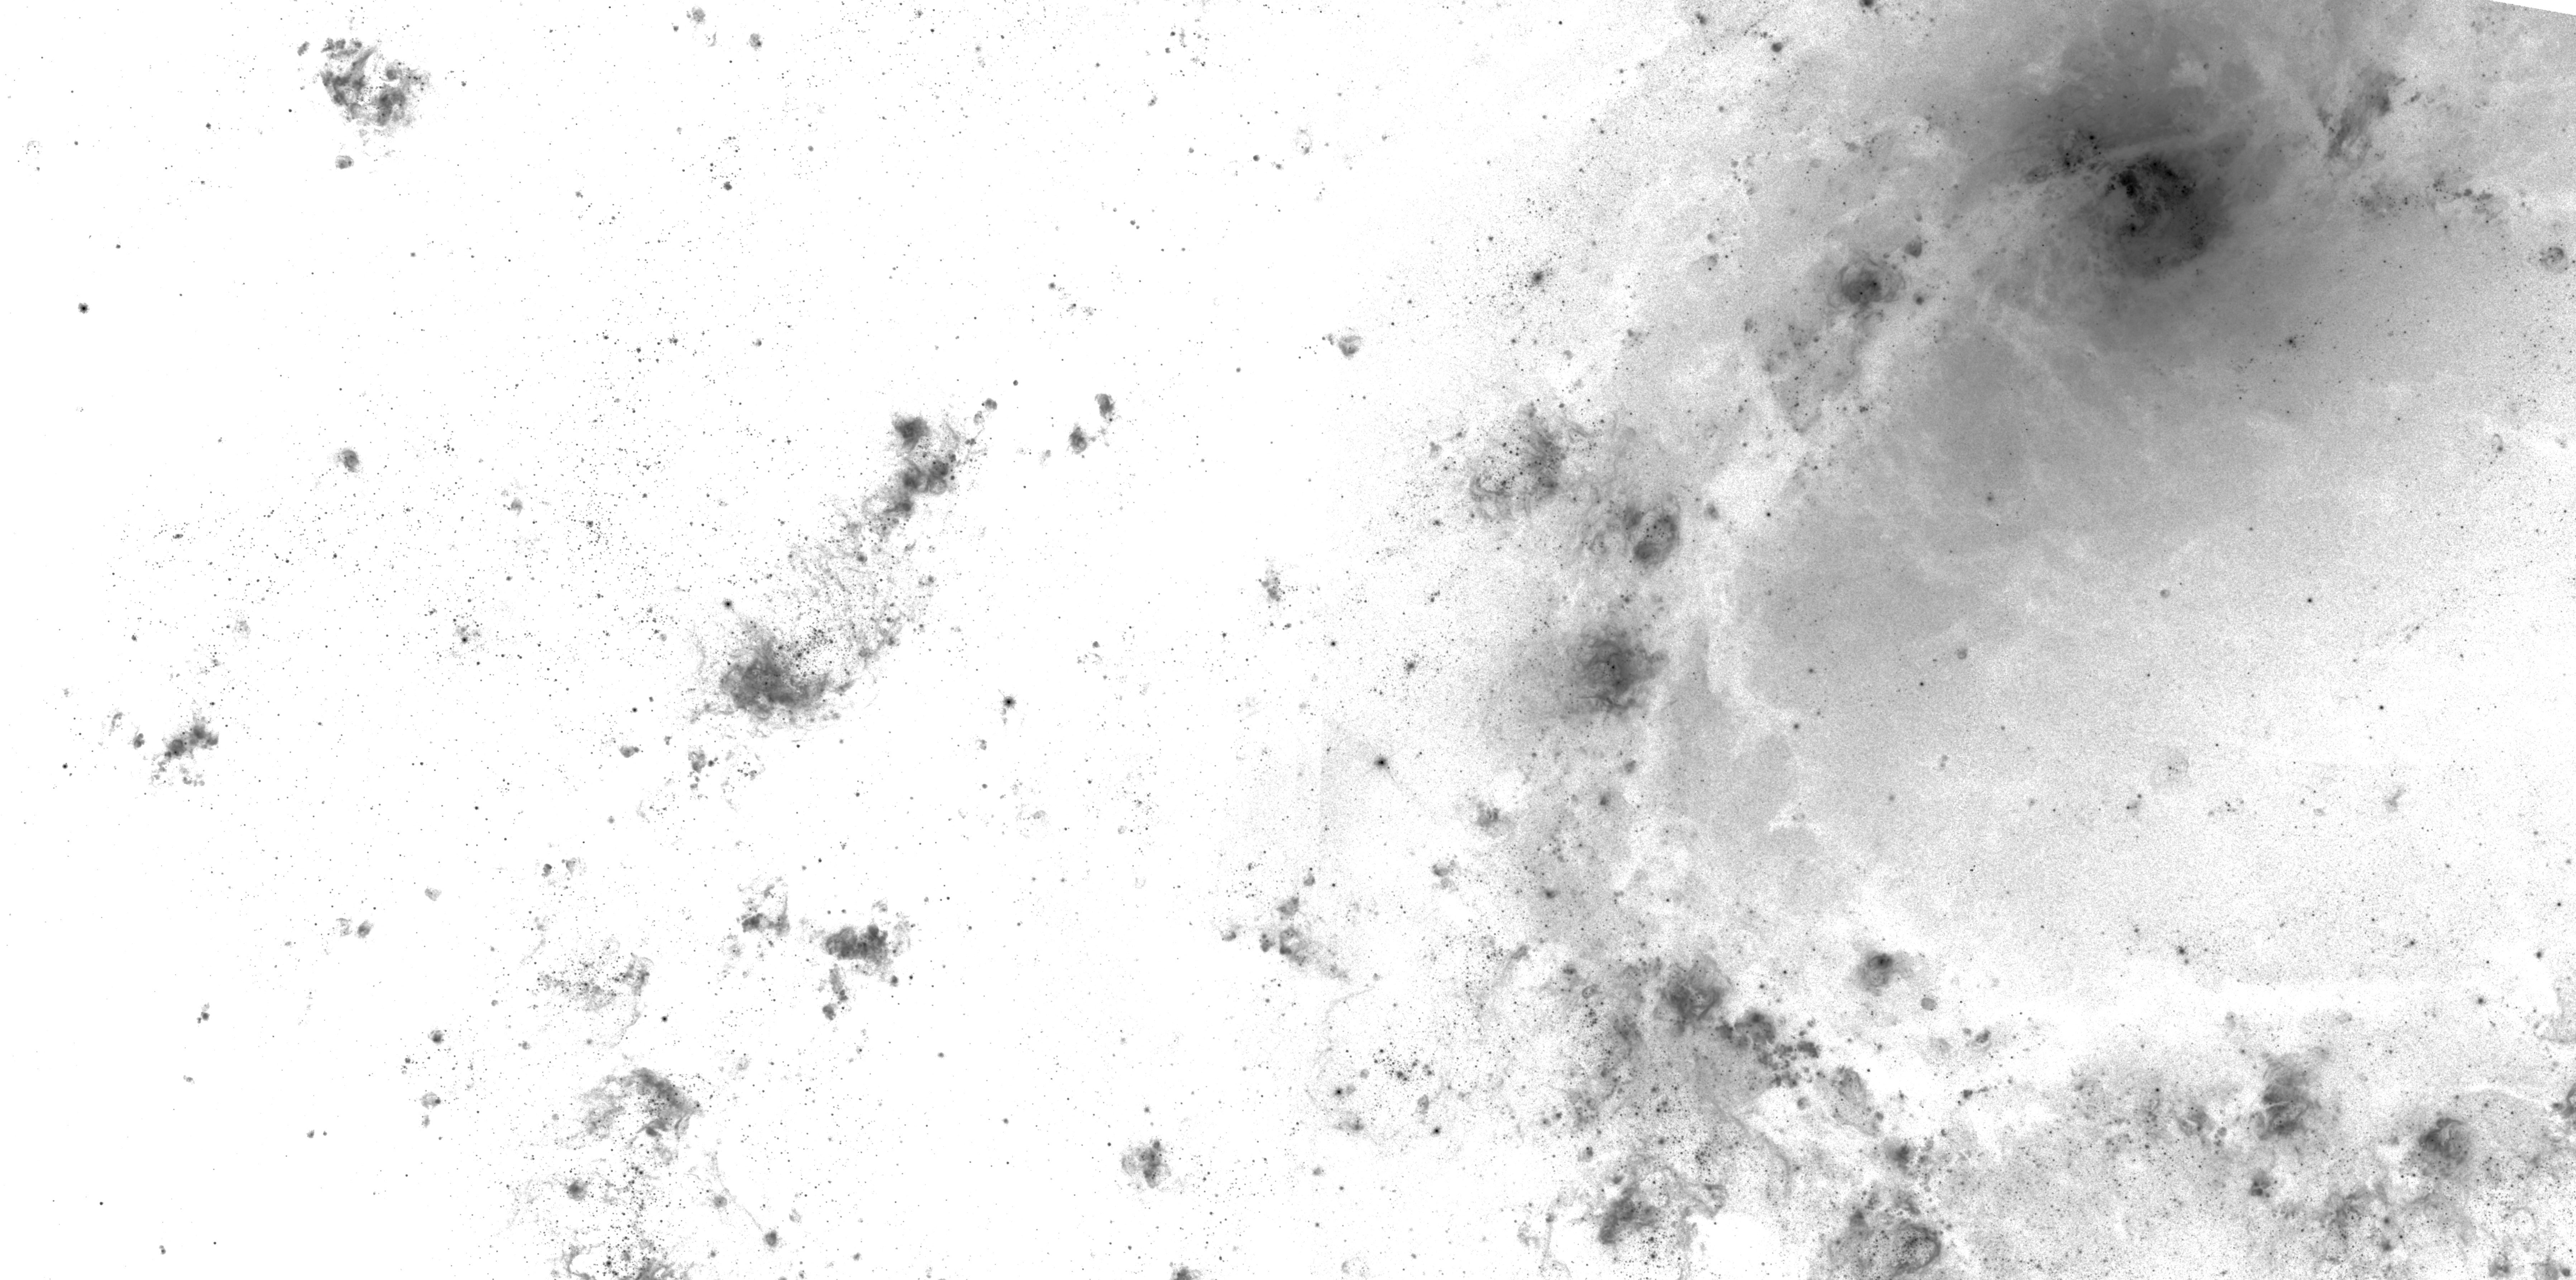
\includegraphics[width=0.77\textwidth]{ha-gray-conv-crp.jpg}
    \caption{Picuture of the M83 galaxy, image taken from the WFC3 ERS M83 Data Products, http://archive.stsci.edu/prepds/wfc3ers/m83datalist.html}
    \label{fig:awesome_image}
\end{figure}

How can we learn something about this image, quantize, get useful information? In the next subsections I will explain the first ideas.

\subsection{Superpixel segmentation}
The main concept of this is to cut an image into bigger neighborhood sections, so from an image that has $425x10^5$ pixels we can get maybe less than 500 superpixels, and then analyse separately those little sections and identify what kind of intersellar objects are they, look at image \ref{fig:super} it is a self-explanatory example of how a superpixel algorithm works.
\begin{figure}[h]
    \centering
    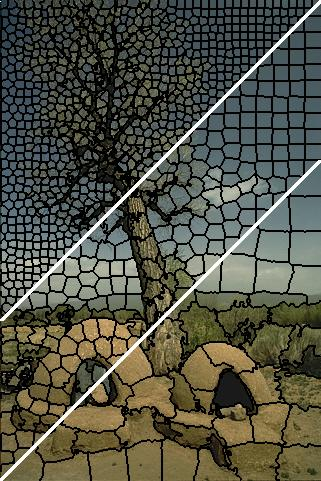
\includegraphics[width=0.37\textwidth]{combo.jpg}
    \caption{Example of a superpixel algorithm}
    \label{fig:super}
\end{figure}
There are many ways to do this and they vary according to color dimensions, methods and number of required superpixels and whether the algorithm is able to find borders and make pixel clasifications.

\begin{remark}
	You can find some example test I tested with Matlab and with Python in this webapage: \url{https://github.com/LaurethTeX/Clustering/blob/master/Methods.md}, also there is a huge amount of information on th internet about this but here are two pages you might find useful:
    \begin{itemize}
    	\item Superpixel: Empirical Studies and Applications \\ \url{http://ttic.uchicago.edu/~xren/research/superpixel/}
        \item Segmentation Algorithms in scikits-image \\ \url{http://peekaboo-vision.blogspot.ca/2012/09/segmentation-algorithms-in-scikits-image.html}
    \end{itemize}
    Also there is one article (from IEEE) I found about and might interest you, it's pure computer science,
    \begin{itemize}
    	\item Normalized Cuts and Image Segmentation \\ \url{http://www.cs.berkeley.edu/~malik/papers/SM-ncut.pdf}
    \end{itemize}
\end{remark}

\subsection{PCA}

Welcome to Astronomy where you will find more acronyms than words to mention something on articles, lots of fun!, well in this case PCA stands for Principal Component Analysis, the objective of this method is to reduce dimnensionality, tranform the data to another space where is can be manipulated and reduced, there are multiple examples of work that has been done in astronomy applying this technique.

Therefor, the idea of applying this method is that if we have multiple-wavelenght images of the same target and transform them to PCA space then we will have less dimensionality and it will be easier to process all the data and fins valuable information.\footnote{Before I forget to mention, later I discovered that PCA is not comonly used for datamining preprocessing because it is hard to interpret the information in the output result. Imagine clusters of data on PCA space, how do you make sense to that?}

\begin{figure}[h]
    \centering
    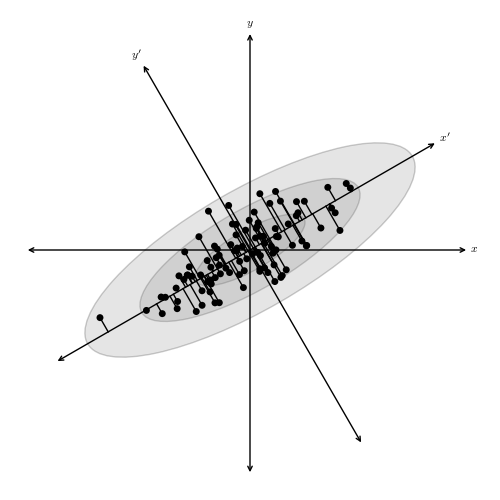
\includegraphics[width=0.37\textwidth]{fig_PCA.png}
    \caption{A distribution of points drawn from a bivariate Gaussian and centered on the origin of $x$ and $y$. PCA defines a rotation such that the new axes ($x’$ and $y’$) are aligned along the directions of maximal variance (the principal components) with zero covariance. This is equivalent to minimizing the square of the perpendicular distances between the points and the principal components}
    \label{fig:pca}
\end{figure}

\begin{remark}
	An example article, where they explain how to apply PCA on multi-wavelenght images and also mentions the pros and cons of using it.
    \begin{itemize}
    	\item Preserving Structure in Multi-wavelength Images of Extended Objects\\ \url{http://arxiv.org/abs/1101.1679v1}
    \end{itemize}
    There's a whole section that talks about this subject with a machine learning approach as a preprocessing step in this nice book,
    \begin{itemize}
    	\item Ivezi{\'c}, \v Z. and Connolly, A.J.
         and Vanderplas, J.T. and Gray, A., \textit{Statistics, Data Mining and Machine Learning in Astronomy}, Princeton University Press, Princeton, NJ, 2014.
    \end{itemize}
\end{remark}

\section{Hypothesis}\index{Hypothesis}
Our data looks like the images on Fig.\ref{fig:cubes}, and it cointains data from let's say a determined galaxy at different wavelengths, if we assume that the galaxy contains various regions that relate to interstellar objects that can tell, how stars are formed, where, how stars die, where was a star, and other mysteries, I guess we can assume that those certain regions can be identified because they share similar characteristics, the ideas is to find how a galaxy is made from, its contents, apply the concept of the superpixel idea in 3D superpixels. 
\begin{figure}[h]
	\centering
    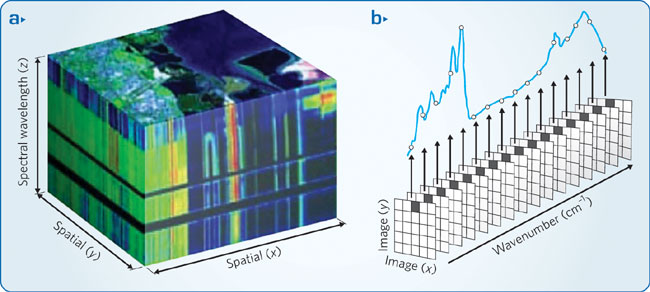
\includegraphics[width=0.57\textwidth]{nphoton.jpg}\hspace{1cm}
    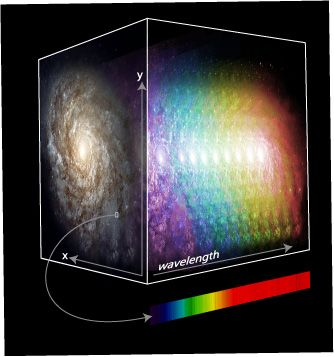
\includegraphics[width=0.27\textwidth]{data.jpg}
    \caption{Illustrations of how a datacube looks like.}
    \label{fig:cubes}
\end{figure}

Take the time to think about this, how the data looks like in 3D, how a star looks like in the datacube, imagine it, this is where ideas of how to tackle this problem come from.
\begin{figure}
	\centering
    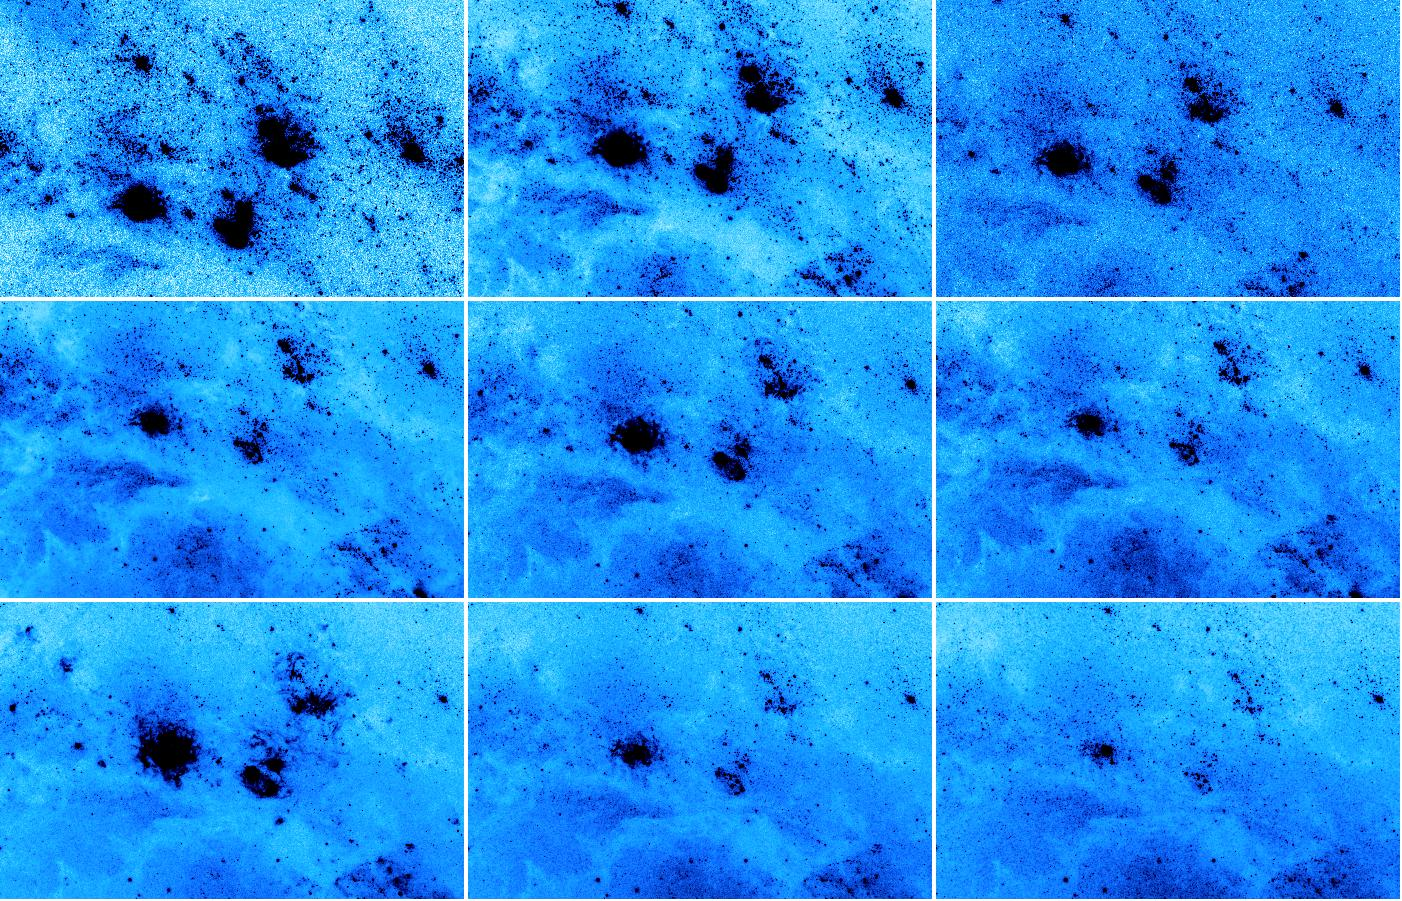
\includegraphics[width=0.87\textwidth]{nine.jpg}
    \caption{Example of how an object can look in 9 wavelenghts}
    \label{fig:nine}
\end{figure}

\subsection{Topics you should review}\index{Related topics}
This will requere a lot of work, but hey it will be worthy and fun!
\begin{itemize}
	\item Astroinformatics and computer science
    	\begin{itemize}
        	\item Data minig
            \item Machine Learning
            \item Big Data Analysis
            \item Neural Networks
            \item Visualization Resources
        \end{itemize}
    \item Statistics and Image Processing
    	\begin{itemize}
        	\item Probability Density Function
            \item Point Spread Function
            \item Full width at half maximum
            \item Convolution
        \end{itemize}
    \item Interstellar medium and star formation
    	\begin{itemize}
        	\item HII regions
            \item Planetary Nebulae
            \item Supernova Remnants
            \item Molecular Gas
            \item All kinds of Nebulae (e.g. dark, refletion)
            \item AGN's (Active Galactic Nucleus)
        \end{itemize}
    \item Astrophysics
    	\begin{itemize}
        	\item Units (light-years, parsecs)
            \item World coordinate system
        	\item Light
            \item Telescopes
            \item Stars and Stellar Evolution
            \item Distance, Brightness, Luminosity
            \item Galaxies
        \end{itemize}
\end{itemize}
The GitHub page will certainly help you to understand why you need to learn about that, and where to find articles, wepages and books.
\subsection{Downloading}
First, let's equip ourselves with the basic software you will need in order to start then you may probably find other cool programs and later you will install them. There is also the possibility that your assigned computer will have them installed already but here is a brief description of what you can do with them, most of them are easy to use.

\begin{description}
	\item[DS9:] It is a program that visualizes astronomy images in FITS format (don't worry if you recognize this format, it will be explained later), where you can easily manipulate them, read their headers, compare, look at regions, see their characteristics, make graphs, even movies. Well, depending on what you need to use later you will be finding all the functions, the best way is to click everywhere and find out what happens, also you can ask to your astronomy colleagues they will tell you all the perks, or if you like learning by yourself or you need someting specific check the documentation webpage. It is faily easy to install, just follow the instructions.
    	\begin{description}
        	\item[Download: ]\url{http://ds9.si.edu/site/Download.html}
            \item[Documentation: ]\url{http://ds9.si.edu/site/Documentation.html}
        \end{description}
        The picture below shows (Fig.\ref{fig:screen}something cool you can do in DS9.
        \begin{figure}[h]
        	\centering
    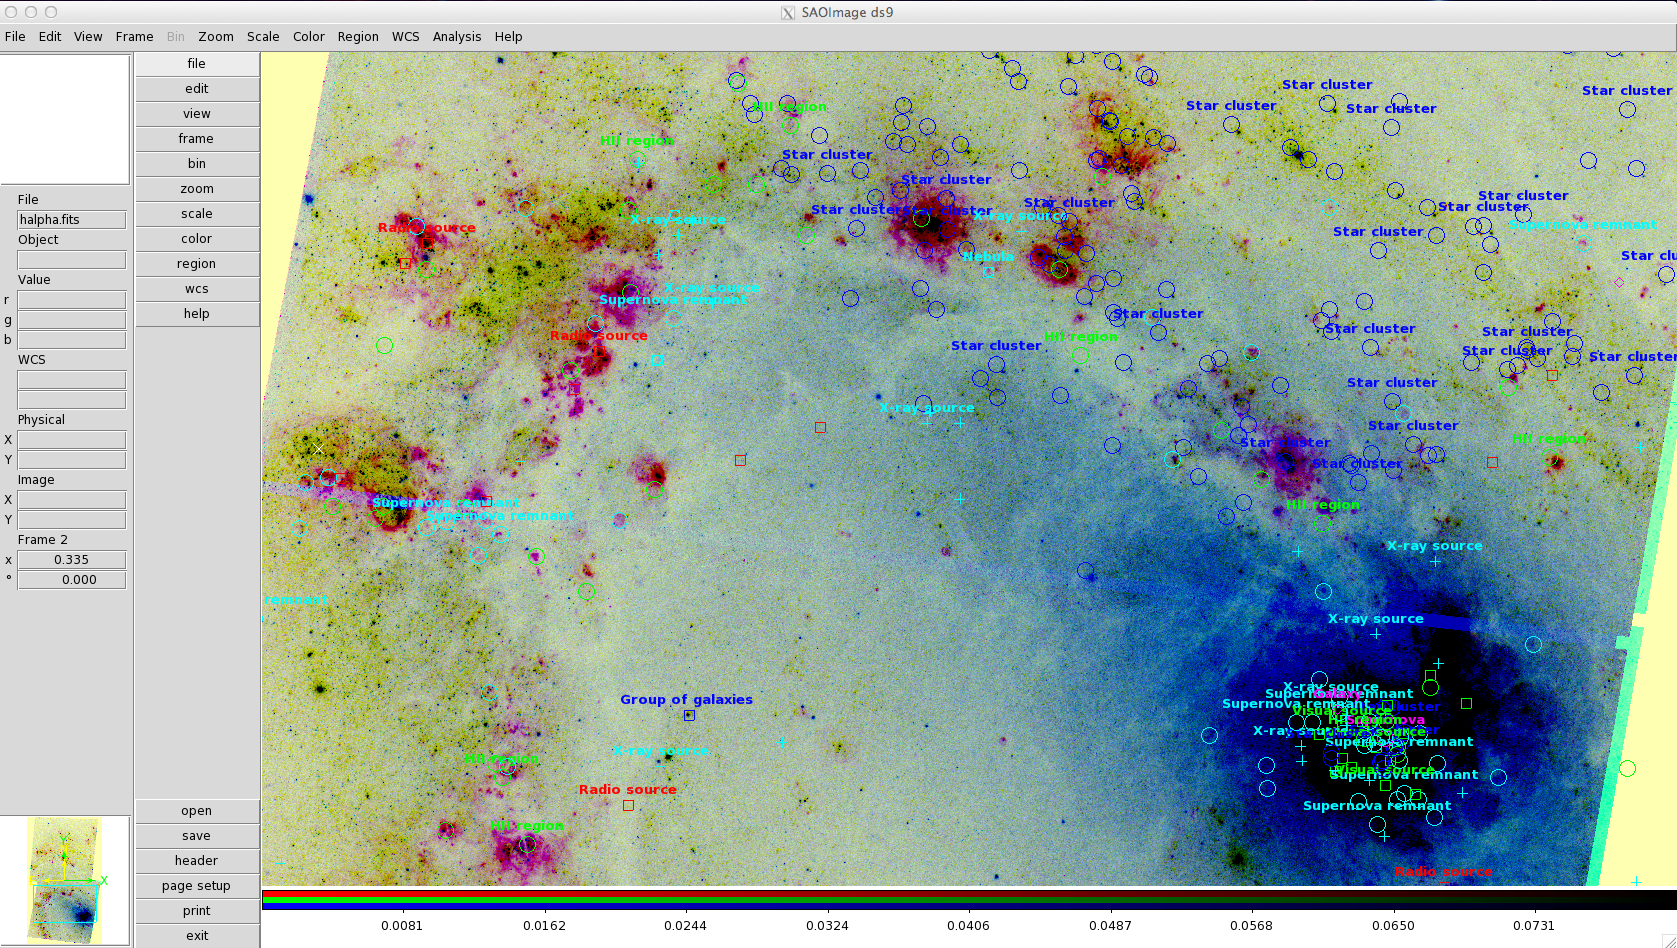
\includegraphics[width=0.87\textwidth]{Screenshot.png}
    \caption{This is an RGB picure made from 3 independent FITS files, with a zscale and a region file overlaid from NED database, if you would like to learn more about this, or reproduce it, it is all explained in this webpage: \url{https://github.com/LaurethTeX/Clustering/blob/master/NEDtoREGION-FILE/KnownRegions.md}}
    \label{fig:screen}
        \end{figure}
        
    \item[Python and a user interface: ]The most \emph{limitless} and user fiendly way to develop programs in Astronomy is using Python, there are many packages, modules, functions now available to help you in almost anything. Me, as an undergrad engineer I'm used to program on an user interface and not directly in a terminal. So, here I will explain you my own way of doing things.
    
    I make my programs on the Canopy editor, it shows when and where you have programing error and warnings, and the interface is easy to learn, now to run, I open a terminal, go to the directory where my program is, type \verb|ipython| wait and then type \verb|run| \verb|myProgram.py|, and wait for the result.
    
    Now there are a lot of fancier ways to work with \emph{Python}, you can program and test directly using \emph{IPython Notebook} on a web broswer or you can just go for the terminal, use \emph{nano} or \emph{vi} or the text editor you like and then run it by typing \verb|python| \verb|myProgram.py|. At this point is up to you, but hey here are some links to start and the packages/modules you should install.
    
    \begin{description}
    	\item[Interfaces or Development environments]\hfill
        	\begin{itemize}
            	\item PyCharm, it a development environment, just like CodeBlocks or NetBeans \url{http://www.jetbrains.com/pycharm/}
                \item Spyder, actually this is the interface that comes with the Python discritution Anaconda, you will get the Python districution and the intrerface. \url{https://store.continuum.io/cshop/anaconda/}
                \item Canopy, this is the one I mentioned before, it super easy to use and you can install packages with one click. \url{https://www.enthought.com/products/canopy/}
            \end{itemize}
        \item[Modules]\hfill
        \\
        In Python, modules are like the libraries in C, therefore, to use math, astronomy and computer science tools you need to install them. To learn whether you already have a module installed or not, type on \emph{iPython} \verb|import andreaModule|, if the output result is something like \verb|ImportError: No module named andreaModule|, you definitely don't have it installed. 
        
        The strategy here to install packages it fairly easy, find their website, go to the download section and follow the instructions, almost all the packages are available on the Python Packaing Index and may be installed by running:
        \begin{verbatim}
        	pip install pyfits
        \end{verbatim}
        To learn how to use them check the documentation page, user manuals or their API's, if you have experience on object oriented programing it will be like running a new bike and if you don't, don't worry too much, Python was designed to be easy to program, just learn the rules of the game.
        	\begin{itemize}
            	\item Astropy, this package is the \emph{must have} of every astronomer, contains tools to handle coordinate systems, units, convolution.. well is better if you take a look at the webpage. \url{http://www.astropy.org/}
                \item Numpy, this package contains the math magic functions, linear algebra tools and the array management variables, make sure you learn all about \emph{Numpy arrays} you will work with them all the time. \url{http://www.numpy.org/}
                \item SciPy, well this package is the base of all scikit modules which contain the functions you will use in image processing and machine learning. \url{http://www.scipy.org/}
                	\begin{itemize}
                    	\item Scikit Image, contains image processing tools, it is the \emph{OpenCV} for \emph{Python} \url{http://scikit-image.org/}
                        \item Scikit Learn, contains data mining algorithms, pretty much contains everything that you will ever need. \url{http://scikit-learn.org/}
                    \end{itemize}
                \item Matplotlib, this package is probably one of the most powerful tools visualize data, you can draw almost anything you want and exacly how you want it. An example of that are the images of the AstroML book, you can access to the image library code and learn how they are made, this is the website \url{http://www.astroml.org/book_figures/index.html}.\footnote{Statistics, Data Mining, and Machine Learning in Astronomy book, it was mentioned before}. You can download the package here \url{http://matplotlib.org/}.
                \item PyFITS, in this package you will find tools to manipulate FITS files, create new ones, create image cubes, tables, and do all kinds of things with their headers. Certainly this package is more than useful. \url{http://www.stsci.edu/institute/software_hardware/pyfits}
            \end{itemize}
    \end{description}
    In the path of researching I'm certain you will find more and new packages and by them you will be prepared to install anything.
    \item[Montage: ]This is a toolkit for assembling astronomical images into mosaics, but it has more functions that you may need in the future to prepare your data before processing it. There are two ways of installing and I would say that is better to have them both. One is to install the toolkit and anytime you need it, you run the commands on the terminal, the other one is to install a \emph{Python} module and use it just like any other module.
    To install montage for terminal, download the lastest version in this website \url{http://montage.ipac.caltech.edu/docs/download.html}, \textbf{read the README file} or go to this website \url{http://montage.ipac.caltech.edu/docs/build.html} and follow the steps, now if you don't have any problem installing it, you can try testing it with an example program found on this website \url{http://montage.ipac.caltech.edu/docs/pleiades_tutorial.html}, in case you are having trouble and your computer is a MAC, instead of doing step five (\emph{If you want to be able to run the Montage executables from any directory}), try this:
    
    \begin{enumerate}
    	\item Open a file called \verb|.profile| located in your user folder. (e.g. \verb|/Users/Laureth|)
        	\begin{verbatim}
            	$ vi .profile
            \end{verbatim}
         \item Include in the file the following
           \begin{verbatim}
           	export PATH=/Applications/Montage_v3.3/bin:$PATH
           \end{verbatim}
           In this link (\url{https://github.com/LaurethTeX/Clustering/blob/master/Tools.md#the-profile-file}) you will find an example of how this file should look. After you modify it, make sure that you save it and type in \verb|/Users/Laureth|,
           \begin{verbatim}
           	$ source .profile
           \end{verbatim}
           Then try testing the \emph{Montage} commands, and I'm sure that it will magically work, just remember that anytime you use any command, type \verb|source .profile|.\\
            
    \end{enumerate}
    
    
    
      Now the other way to install, implies only to install a \emph{Python} module but this module contains less functions that the terminal application, in any case check the website \url{http://www.astropy.org/montage-wrapper/}, there you will find all the documentation you may need and the instructions to install it (\emph{Spoilers} \verb|pip install montage-wrapper| ).\\
\end{description}

Any questions you may have and how to install, here is my GitHub page for software tools \url{https://github.com/LaurethTeX/Clustering/blob/master/Tools.md}


\vfill
\textit{Wish you all the best, Andrea Hidalgo}
\end{document}